\documentclass[11pt]{article}
\usepackage[T1]{fontenc}
\usepackage[a4paper,margin=2.1cm]{geometry}
\usepackage{amsmath,amssymb,booktabs,graphicx,float,tikz,array,enumitem,pifont}
\usepackage[most]{tcolorbox}
\usepackage[hidelinks]{hyperref}
\usetikzlibrary{positioning,arrows.meta,calc,shapes.misc}

\definecolor{ink}{HTML}{1B2430}
\definecolor{ink2}{HTML}{4A5462}
\definecolor{trace}{HTML}{2A78D6}
\definecolor{image}{HTML}{C9551F}
\definecolor{model}{HTML}{13865D}
\definecolor{problem}{HTML}{B3372E}
\definecolor{gold}{HTML}{B8860B}

\setlength{\parindent}{0pt}
\setlength{\parskip}{0.55em}
\setlist{itemsep=0.15em,topsep=0.3em}
\renewcommand{\familydefault}{\sfdefault}

% the three parts under every figure
\newcommand{\readit}[1]{\par\textcolor{trace}{\textbf{How to read it.}} #1\par}
\newcommand{\shows}[1]{\par\textcolor{ink}{\textbf{What it shows.}} #1\par}
\newtcolorbox{point}{colback=model!8,colframe=model!70,boxrule=0.6pt,arc=2pt,left=6pt,right=6pt,top=4pt,bottom=4pt,fontupper=\small}
\newtcolorbox{caveat}{colback=problem!6,colframe=problem!60,boxrule=0.6pt,arc=2pt,left=6pt,right=6pt,top=4pt,bottom=4pt,fontupper=\small}
\newcommand{\figw}[2][0.82]{\begin{center}\includegraphics[width=#1\linewidth]{figures/#2.png}\end{center}\vspace{-0.6em}}
\newcommand{\q}[1]{\textit{Question: #1}\par}
\newcommand{\cmark}{\textcolor{model}{\ding{51}}}
\newcommand{\xmark}{\textcolor{problem}{\ding{55}}}

\tikzset{
  box/.style={draw=#1,fill=#1!8,rounded corners=3pt,align=center,font=\small,minimum height=1.0cm,text width=2.5cm,line width=0.8pt},
  box/.default=ink2,
  arr/.style={-{Stealth[length=2.5mm]},line width=0.9pt,color=ink2},
}

\title{\textbf{Level 1, explained}\\[4pt]\large Can a two-second readout trace tell us which CCD settings are good?\\
What we did on the first night of data, what we learned, and what the next data taking is for}
\author{ccd\_opt\_ml}
\date{2026-11-05}

\begin{document}
\maketitle
\thispagestyle{empty}

\section*{The whole story on one page}

\begin{enumerate}[leftmargin=1.4em]
\item \textbf{The goal.} Finding good settings for a skipper CCD means trying many settings, and every try costs a
  $\sim$10-minute image. A \emph{trace} (2 seconds of raw readout) is cheap. Can the trace tell us what the image would
  show?
\item \textbf{The data.} One night, 43 \emph{packets}. Each packet sets one combination of settings and records traces
  and one image. The image gives the true read noise $\sigma_e$, dark charge $\lambda$ and gain.
\item \textbf{One trace $\to$ the image's numbers.} On the amplifiers the model was trained on, it works. On a separate
  test session the error for $\lambda$ fell from 23\,\% (no trace) to 5\,\%, and for $\sigma_e$ from 10 to 7\,\%.
\item \textbf{But part of that is recognising the amplifier.} Each of the four amplifiers has its own level, and many
  trace features are just ``fingerprints'' of which amplifier it is. On an amplifier the model never saw, it cannot
  predict the level.
\item \textbf{So compare two traces of the same amplifier instead.} The amplifier's own level cancels in a comparison.
  ``Is setting B better than setting A?'' is answered correctly about 75--90\,\% of the time, even on an amplifier the
  model never saw.
\item \textbf{The funnel.} Compare every pair of 100 candidate settings, sort them like a tournament, and take images
  of only the top 5. Replayed on the first night (35 settings), the model's order matches the true order well
  (rank correlation 0.85), but the single best setting came 7th.
\item \textbf{v2.} The next data taking fixes what the first night got wrong: settings varied jointly instead of one at
  a time, a small \emph{level-1 strip} in every packet that measures the amplifier's level directly, more and checked
  data, and a real test of the funnel on 100 new settings.
\end{enumerate}

\begin{center}
\resizebox{\linewidth}{!}{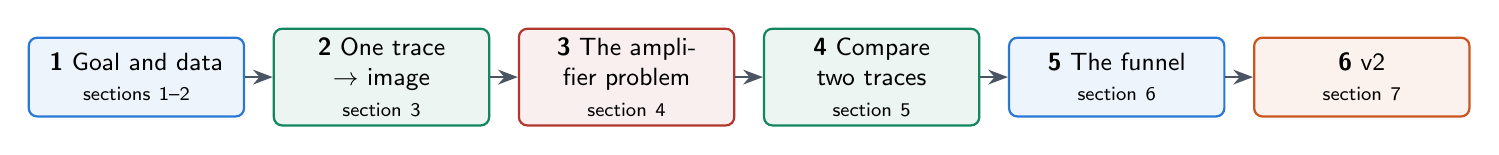
\begin{tikzpicture}[node distance=0.35cm]
\node[box=trace] (a) {\textbf{1} Goal and data\\\scriptsize sections 1--2};
\node[box=model,right=of a] (b) {\textbf{2} One trace $\to$ image\\\scriptsize section 3};
\node[box=problem,right=of b] (c) {\textbf{3} The amplifier problem\\\scriptsize section 4};
\node[box=model,right=of c] (d) {\textbf{4} Compare two traces\\\scriptsize section 5};
\node[box=trace,right=of d] (e) {\textbf{5} The funnel\\\scriptsize section 6};
\node[box=image,right=of e] (f) {\textbf{6} v2\\\scriptsize section 7};
\foreach \x/\y in {a/b,b/c,c/d,d/e,e/f} \draw[arr] (\x)--(\y);
\end{tikzpicture}}
\end{center}

\subsection*{Words used in this document}
\small
\begin{tabular}{>{\bfseries}p{3.3cm}p{12.6cm}}
\toprule
trace & 2 seconds of raw readout of 10 pixels, every ADC sample kept. Cheap.\\
image & a full readout (16 rows $\times$ 1000 columns, 500 skips per pixel), $\sim$10 minutes. Gives the truth.\\
setting / knob & the CCD's operating parameters: timing (e.g.\ delayInt) and voltages (e.g.\ VR, VDD).\\
nominal & the standard setting everything is compared with.\\
packet & one setting: traces before the change (at nominal), the change, traces after it, one image.\\
amplifier (ch0--ch3) & the CCD has four output amplifiers read at the same time; each gives its own numbers.\\
$\sigma_e$, $\lambda$, gain & read noise (electrons), dark charge (electrons per pixel), gain (ADU per electron); see section~\ref{sec:hist}.\\
label & the true value of $\sigma_e$, $\lambda$ or gain, measured from the image.\\
label noise & how much a label changes when the \emph{same} setting is measured twice.\\
error (\%) & how far a prediction typically is from the label; 10\,\% means ``off by a factor of about 1.1''.\\
known / new amplifier & tested on an amplifier that was in the training data / one that was left out.\\
fingerprint & a trace feature whose value mostly says \emph{which amplifier} it is.\\
absolute model & one trace in, the image's $\sigma_e$, $\lambda$, gain out.\\
change model & two traces in, ``how does B differ from A?'' (or just ``is B better?'') out.\\
direction & whether a change is up or down; ``direction right'' is the share of real changes called the right way.\\
rank correlation & how well an order matches the true order: 1 = perfect, 0 = random.\\
screen / shortlist & a trace-only test of one setting / the few settings picked to be imaged.\\
strip & a tiny image (2 rows) read exactly like the real image, with every skip kept.\\
\bottomrule
\end{tabular}
\normalsize

\clearpage
% =====================================================================================================
\section{The goal: replace most images with traces}

\subsection{Every setting we try costs an image}
To tune a CCD we change its settings and look at what happens to the noise. The only trustworthy way to see what
happens is to take an image and fit it, which takes about 10 minutes per setting. Trying hundreds of settings that way
takes days.

A \textbf{trace} is a 2-second recording of the raw readout of a few pixels. If a trace can tell us what the image
\emph{would} show, we can try many settings with traces and only take images of the most promising ones.

\begin{center}
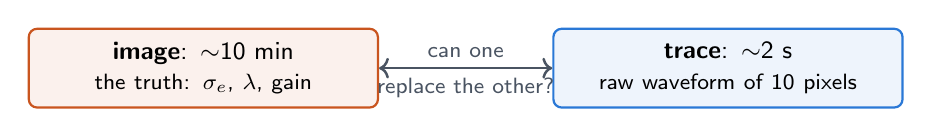
\begin{tikzpicture}[node distance=0.6cm]
\node[box=image,text width=4.2cm] (i) {\textbf{image}: $\sim$10 min\\\footnotesize the truth: $\sigma_e$, $\lambda$, gain};
\node[box=trace,right=2.2cm of i,text width=4.2cm] (t) {\textbf{trace}: $\sim$2 s\\\footnotesize raw waveform of 10 pixels};
\draw[arr,<->] (i) -- node[above,font=\footnotesize] {can one} node[below,font=\footnotesize] {replace the other?} (t);
\end{tikzpicture}
\end{center}

\subsection{What we want to predict: three numbers read off the image}\label{sec:hist}
\figw[0.8]{e_histogram}
\readit{An illustration of an image's pixel values. Every pixel holds a whole number of electrons (mostly 0,
sometimes 1 or 2). The readout adds noise, so each electron count becomes a bump.}
\shows{The three numbers we care about are read directly off this picture:
\textcolor{problem}{read noise $\sigma_e$} is the width of a bump (smaller is better),
\textcolor{model}{gain} is the distance between bumps (it converts the readout's units, ADU, into electrons), and
\textcolor{image}{dark charge $\lambda$} is the share of pixels that caught a stray electron (smaller is better).}

\subsection{What a trace is}
\figw[0.95]{e_trace_schematic}
\readit{Left: one ``skip'' of the raw waveform (an illustration). The electronics measure a baseline
(\textcolor{trace}{pedestal window}), move the pixel's charge in, and measure again (\textcolor{image}{signal window}).
Signal minus pedestal is one measurement of the pixel. Right: a skipper CCD repeats this 500 times for every pixel.}
\shows{One measurement is very noisy (spread $w\approx5.6$ ADU, the ``white noise per skip''). The average of 500 is
much less noisy, roughly $5.6/\sqrt{500}=0.25$ ADU. The image keeps only that average. The trace keeps every raw
sample of a few pixels, so it shows the noise itself. From each trace we compute 141 numbers (``features''), such as
the white noise per skip, ringing after the reset pulse and slow drifts, plus 16 curves.}

\subsection{How the data were taken}
\begin{center}
\resizebox{0.95\linewidth}{!}{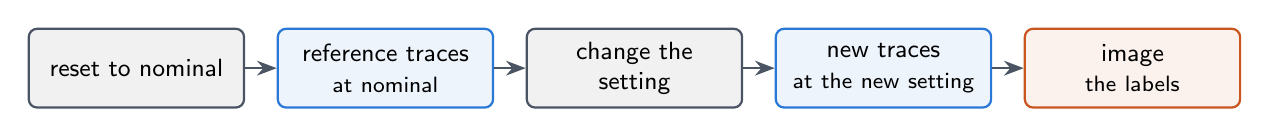
\begin{tikzpicture}[node distance=0.4cm]
\node[box] (a) {reset to nominal};
\node[box=trace,right=of a] (b) {reference traces\\\footnotesize at nominal};
\node[box,right=of b] (c) {change the setting};
\node[box=trace,right=of c] (d) {new traces\\\footnotesize at the new setting};
\node[box=image,right=of d] (e) {image\\\footnotesize the labels};
\foreach \x/\y in {a/b,b/c,c/d,d/e} \draw[arr] (\x)--(\y);
\end{tikzpicture}}
\end{center}
One \textbf{packet} = one setting. The night of 2026-11-02 had 43 packets in three sessions:
\begin{itemize}
\item \textbf{Session A} (17 packets): timing knobs, one at a time.
\item \textbf{Session B} (15 packets): voltages, one at a time.
\item \textbf{Session C} (11 packets): several knobs changed together. Kept \emph{sealed}: not looked at until the
  models were chosen, then used once as the honest test.
\end{itemize}
Four amplifiers are read at once, so every packet gives four rows of data. We used board 101. Its ch2 turned out to
behave oddly (section~\ref{sec:amp}) and is left out of most results. Three session-C packets lost their traces, which
left 8 usable test packets.

% =====================================================================================================
\section{How good are the measurements we learn from?}

\subsection{For $\lambda$ and gain, a typical knob effect is no bigger than the measurement noise}
\q{if we measure the same setting twice, how different are the two answers, compared with what a knob actually does?}
\figw[0.9]{e_label_noise}
\readit{For each number, grey is how much the label changes when the \emph{same} setting is measured twice, and blue is
the typical change caused by turning one knob.}
\shows{For $\sigma_e$ a knob's effect (3.9\,\%) is twice the noise (1.9\,\%), so changes are easy to see. For $\lambda$
(8.5 vs 11.9\,\%) and the gain (0.4 vs 0.8\,\%), a typical knob effect is \emph{smaller} than the noise.}
\begin{point}
Any score of ``did the model get the change right?'' has to count only \textbf{clear changes}, ones larger than the
noise. Otherwise it would be grading the model on coin flips. That is how every direction score below is computed.
\end{point}

\subsection{$\lambda$ drifts during the night even when nothing is changed}
\figw[0.75]{e_lambda_drift}
\readit{Only the packets at the nominal setting, one line per amplifier, against the time of night.}
\shows{Nothing was changed between these packets, yet $\lambda$ moved: ch0 fell 22\,\%, ch1 15\,\%. Dark charge
depends on the CCD's recent history (how long since it was last cleared), not only on the settings. One packet
(L1\_18) waited 38 minutes before its image without a clear, and its $\lambda$ came out four times too high.}
\begin{point}
Part of $\lambda$ cannot be predicted from settings or traces at all. The next data taking clears the CCD right before
every image and repeats the nominal setting every 7 packets to track the drift.
\end{point}

\subsection{A processing error was found and fixed before any conclusions}
Our image processing at first applied a ``drift correction'' to every image. Two packets with the \emph{same} setting
(L1\_06 and L1\_23) then disagreed by 60\,\% in $\sigma_e$, while their traces agreed. Running the fit on the raw
images showed the correction itself was the problem: it tripled $\sigma_e$ in places (L1\_03 ch0: 0.24 $\to$ 0.69).
It was switched off, all 43 packets were reprocessed, and every result below uses the corrected labels. Repeating a
setting is the cheapest check of the labels, which is why v2 repeats settings away from nominal too.

% =====================================================================================================
\section{Predicting the image from one trace}

\subsection{How we tested honestly}
\begin{center}
\resizebox{0.9\linewidth}{!}{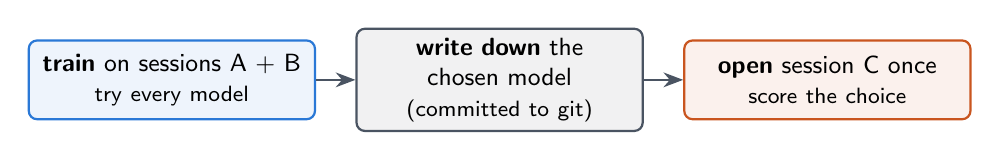
\begin{tikzpicture}[node distance=0.5cm]
\node[box=trace,text width=3.4cm] (a) {\textbf{train} on sessions A + B\\\footnotesize try every model};
\node[box,right=of a,text width=3.4cm] (b) {\textbf{write down} the chosen model\\\footnotesize (committed to git)};
\node[box=image,right=of b,text width=3.4cm] (c) {\textbf{open} session C once\\\footnotesize score the choice};
\draw[arr] (a)--(b); \draw[arr] (b)--(c);
\end{tikzpicture}}
\end{center}
While choosing, models are compared by \emph{cross-validation}: hold out a few packets, train on the rest, predict
the held-out ones, and repeat. The test session C stays untouched until the choice is fixed, so the final score cannot
be tuned to it. About 17 models were tried (all listed in the appendix). They range from ``no trace at all'' (guess
from the settings and which amplifier it is), through models built on the physics of the readout, to flexible
machine-learning models (boosted trees, Gaussian processes, neural networks).

\subsection{On the sealed test, the trace clearly helps for $\lambda$}
\figw[0.9]{e_session_c}
\readit{Typical error on session C. Grey: the best model that sees \emph{no trace}, only the settings and which
amplifier. Blue: the best model using the trace. ``Significant'' means the improvement holds when the 8 test packets
are resampled.}
\shows{$\lambda$: 23\,\% $\to$ 5\,\%, a large and significant gain. $\sigma_e$: 10 $\to$ 7\,\%, gain: 1.4 $\to$
0.9\,\%. Both are better, but with only 8 test packets not significant. The winning model in all three is the
\emph{physics-structured} one (next figure).}

\subsection{Why $\sigma_e$ works: the trace measures it almost directly}
\figw[0.6]{e_physics_white}
\readit{Each dot is one packet on one amplifier. x: $\sigma_e$ computed from the trace alone, white noise per skip
$w$ divided by $\sqrt{500}$ and by the gain. y: $\sigma_e$ from the image. Colour: what kind of setting was changed.}
\shows{For voltage changes (blue) the dots sit on one line: the image's noise is about 0.81 $\times$ what the trace
measures, at every setting. The model ``physics\_white'' is exactly this measurement plus small learned corrections.
That is why it carries over to new settings. Timing changes (orange) scatter above the line: they make the image
noisier in ways the trace does not see. The trace reads 10 pixels after a short burst, while the image reads
$10^4$ pixels after a long ``prescan'' and a clear. This gap is one reason for the strips in v2.}

\subsection{The training check picked the wrong model}
\figw[0.65]{e_cv_vs_c}
\readit{$\sigma_e$ error of five models, measured twice. Left: the training check (cross-validation on A+B), used to
choose. Right: the sealed test. Lower is better (the axis is flipped so ``better'' is up).}
\shows{The model that looked best in training (gp\_dim, red) became the worst on the test. The physics model (green)
went from middle to best. The reason: sessions A and B changed one knob at a time, so holding out a packet asked
models to predict a knob value they had never seen move, i.e.\ to \emph{extrapolate}. Session C moved all knobs inside
their ranges, which is \emph{interpolation}. Flexible models extrapolate badly; the physics model extrapolates well.}
\begin{point}
The data used for choosing must look like the data the model will face. v2 changes all knobs together in every
packet, so training and test ask the same kind of question.
\end{point}

% =====================================================================================================
\section{The amplifier problem}\label{sec:amp}

\subsection{Each amplifier has its own level}
\figw[0.9]{e_amp_levels}
\readit{The nominal-setting packets only (same setting), split by amplifier.}
\shows{At the same setting, the four amplifiers give clearly different numbers: $\sigma_e$ 0.15 (ch0) to 0.18 (ch3),
$\lambda$ 0.25 to 0.65, gain 1.26 to 1.35. ch2 (purple) is the odd one out in $\lambda$, and its fits were poor; it is
left out of most results.}
\begin{point}
A model that only works out \emph{which} amplifier it is looking at already predicts a lot. So the fair baseline is
``settings + which amplifier, no trace'', and that is the grey bar in every comparison above.
\end{point}

\subsection{Many trace features are amplifier fingerprints}
\figw[0.92]{e_fingerprint}
\readit{Two trace features over the night, coloured by amplifier (log scale). Left: the size of the ringing after the
reset pulse in the reference trace. Right: the white noise per skip.}
\shows{Left: each amplifier sits on its own flat band all night, whatever the setting. This feature tells you
\emph{which amplifier} it is and nothing about the setting: a \textbf{fingerprint}. Right: the white noise overlaps
between amplifiers and moves with the settings. That is useful information. Of 141 features, 52 behave like the left
panel (more than 90\,\% of their variation is ``which amplifier''). Almost all of them come from the reference trace,
which is always taken at nominal.}

\subsection{On an amplifier the model never saw, the level is lost}
\figw[0.9]{e_new_amp}
\readit{Typical error of the best trace model on an amplifier that was in the training data (blue), on one that was
left out (orange), and of simply guessing the average of the other amplifiers (grey).}
\shows{On a new amplifier the errors grow a lot, and for $\lambda$ and gain they are close to just guessing the
average. Removing the fingerprint features confirms it: on the sealed test the $\lambda$ error rose from 5 to 15\,\%
and the gain error from 0.9 to 2.8\,\%, while $\sigma_e$ did not change. For $\lambda$ and gain, much of the earlier
success was the model \emph{recognising} the amplifier.}

\subsection{Why: a trace cannot tell noise from gain}
The trace measures in ADU, the readout's own unit, and contains no known amount of charge. Its noise is
\[\text{noise in ADU}=\sigma_e\times\text{gain}.\]
An amplifier with $\sigma_e=0.15$ and gain 1.34 gives the same trace noise as one with $\sigma_e=0.16$ and gain 1.26.
The trace cannot separate them; only whole electrons can (the spacing of the bumps in section~\ref{sec:hist}). On a known
amplifier the model gets around this by recognising it. On a new one it cannot.

\subsection{One measurement per amplifier fixes the level}
We also tested on a second board (102), with models trained only on board 101. The models' predictions for 102 were
off, and off by about the same amount on every packet: they had the wrong \emph{level} for this new board.

\textbf{What ``one calibration image'' means.} Take the first image of board 102 and see how far off each model was
on it. That miss is the board's level offset. Then correct every \emph{later} prediction for that amplifier by the
same amount (in log units, i.e.\ multiply by the same factor), and score the corrected predictions on the remaining
packets:
\[\text{corrected prediction}=\text{model's prediction}\times\frac{\text{value measured on the calibration image}}{\text{model's prediction for that image}}.\]

\begin{center}\small
\begin{tabular}{lcc}\toprule
 & before the calibration & after one calibration image\\\midrule
$\sigma_e$ & physics model 30\,\% too low & $\sim$11\,\% (the label scatter of that board)\\
$\lambda$ & most models $\sim$90\,\% too low & $\sim$8\,\%\\
gain & 2--8\,\% too high & 0.3\,\%\\\bottomrule
\end{tabular}
\end{center}
After the correction every model is as close as the labels themselves repeat, so the remaining error is measurement
noise.
\begin{caveat}
Board 102 stayed at the nominal setting all night (only board 101's settings were changed). So this shows that one
image fixes a new board's level and that the level then stays put. It does \emph{not} show that the model follows
setting changes on a new board, because nothing changed. That needs a second CCD whose settings are varied (planned
after v2).
\end{caveat}
\begin{point}
The trace predicts \emph{how the numbers move} when settings change. It cannot predict \emph{where an amplifier
starts}. That has to be measured once, by an image or (in v2) by a strip. This leads directly to the next idea: if we
only ever compare two traces of the same amplifier, the starting level is not needed at all.
\end{point}

% =====================================================================================================
\section{Comparing two traces instead of predicting one}

\subsection{The idea: the amplifier's level cancels in a comparison}
\figw[0.72]{e_offset_toy}
\readit{An illustration. Amplifier A (blue) and amplifier B (orange) start at different levels. Going from setting 1 to
setting 2 lowers both by 20\,\%.}
\shows{A model that predicts the \emph{value} and was trained on A answers ``0.24'' for B: it learned A's level and is
wrong. A model that predicts the \emph{change} (``20\,\% lower'') is right for both, because the level drops out of a
difference:
\[\log\lambda_B-\log\lambda_A=\bigl(\text{level}+f(\text{trace B})\bigr)-\bigl(\text{level}+f(\text{trace A})\bigr)=f(\text{trace B})-f(\text{trace A}).\]
This \textbf{change model} takes two traces of the same amplifier and outputs how $\sigma_e$, $\lambda$ and gain
differ between them. It is also exactly what tuning needs: ``is the new setting better than the current one?''}

\subsection{A worked example: two real packets}
The change model is given the 141 features of trace A, the 141 features of trace B, and their differences. Here it is
on two pairs of first-night packets, on amplifier ch0, with a model that was \emph{never trained on ch0}:

\begin{center}
\resizebox{\linewidth}{!}{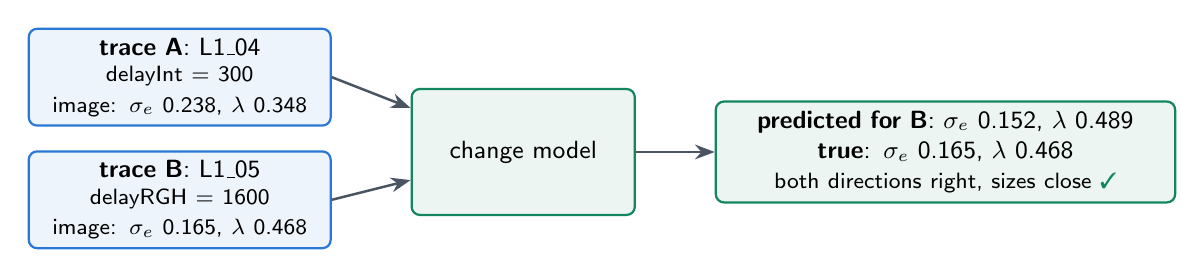
\begin{tikzpicture}[node distance=0.45cm]
\node[box=trace,text width=3.6cm] (a) {\textbf{trace A}: L1\_04\\\footnotesize delayInt = 300\\image: $\sigma_e$ 0.238, $\lambda$ 0.348};
\node[box=trace,below=0.3cm of a,text width=3.6cm] (b) {\textbf{trace B}: L1\_05\\\footnotesize delayRGH = 1600\\image: $\sigma_e$ 0.165, $\lambda$ 0.468};
\node[box=model,right=1.0cm of a,yshift=-0.95cm,text width=2.6cm,minimum height=1.6cm] (m) {change model};
\node[box=model,right=1.0cm of m,text width=5.6cm] (o) {\textbf{predicted for B}: $\sigma_e$ 0.152, $\lambda$ 0.489\\\textbf{true}: $\sigma_e$ 0.165, $\lambda$ 0.468\\\footnotesize both directions right, sizes close \cmark};
\draw[arr] (a.east)--(m); \draw[arr] (b.east)--(m); \draw[arr] (m)--(o);
\end{tikzpicture}}

\vspace{0.6em}
\resizebox{\linewidth}{!}{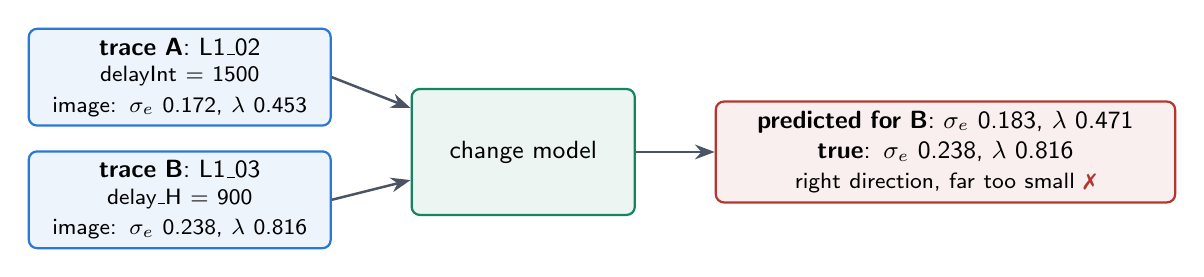
\begin{tikzpicture}[node distance=0.45cm]
\node[box=trace,text width=3.6cm] (a) {\textbf{trace A}: L1\_02\\\footnotesize delayInt = 1500\\image: $\sigma_e$ 0.172, $\lambda$ 0.453};
\node[box=trace,below=0.3cm of a,text width=3.6cm] (b) {\textbf{trace B}: L1\_03\\\footnotesize delay\_H = 900\\image: $\sigma_e$ 0.238, $\lambda$ 0.816};
\node[box=model,right=1.0cm of a,yshift=-0.95cm,text width=2.6cm,minimum height=1.6cm] (m) {change model};
\node[box=problem,right=1.0cm of m,text width=5.6cm] (o) {\textbf{predicted for B}: $\sigma_e$ 0.183, $\lambda$ 0.471\\\textbf{true}: $\sigma_e$ 0.238, $\lambda$ 0.816\\\footnotesize right direction, far too small \xmark};
\draw[arr] (a.east)--(m); \draw[arr] (b.east)--(m); \draw[arr] (m)--(o);
\end{tikzpicture}}
\end{center}
The predicted value is trace A's measured value times the predicted change. The second case is a miss: delay\_H = 900
made the image much worse in a way the trace barely shows. That is the same timing gap as in the $\sigma_e$ figure of
section 3.

\subsection{Proof that the level cancels: the odd amplifier ch2}
\figw[0.78]{e_ch2}
\readit{ch2 is the amplifier with the unusual $\lambda$. Here every model was trained on the other three amplifiers
and asked about ch2. Each bar is how far off the model is on average.}
\shows{Every model that predicts the \textbf{level} (red) misses ch2 by 54--100\,\%, because ch2's level is unlike
anything it was trained on. Every model that predicts the \textbf{change} (green) is off by at most 7\,\%. The level
cancels, as the formula says. A practical bonus: ch2's data hurt the level models but can safely be used to train the
change models.}

\subsection{How often the comparison is right}
\figw[0.75]{e_direction}
\readit{Pairs of packets on an amplifier the model never saw. For every clear change, did the model say the right
direction (better or worse)? Grey: a model that only looks at the two settings, no traces. Blue: the best change
model.}
\shows{Using traces, the direction is right 75\,\% of the time for $\sigma_e$, 89\,\% for $\lambda$ and 88\,\% for the
gain, versus 68--75\,\% from the settings alone. The best version gives the model trace A, trace B \emph{and} their
difference. It can then learn things like ``this change matters more when A is already noisy''. These gains are not
yet statistically firm: there were only about 50--120 clear changes per number.}

\subsection{A trap we fell into: ``always say worse'' scores 96\,\%}
\figw[0.6]{e_always_up}
\readit{The share of clear $\sigma_e$ changes that go up (get worse). Left: from nominal to the packet's new setting.
Right: from one packet to the next.}
\shows{Nominal is already a good setting, so moving away from it almost always makes $\sigma_e$ worse (96\,\%). A
model that always answers ``worse'' scores 96\,\% there without looking at the traces. An earlier result
(``94\,\% right'') was mostly this. The fix: always test on pairs that go up and down equally often (packet to next
packet, 52\,\%), and train on every pair in both orders. In v2, a third of the packets compare with the
\emph{previous packet's} setting instead of nominal.}

\subsection{Which kinds of change does it work for?}
\begin{center}\small
\begin{tabular}{lccc}\toprule
pair of traces that differ in & $\sigma_e$ & $\lambda$ & gain\\\midrule
nominal vs a timing change & \cmark\ 88\,\% & \cmark\ 100\,\% & too few\\
nominal vs an output-stage voltage (VDD, VR, RG, SW) & too few & too few & \cmark\ 89\,\%\\
nominal vs clock-rail voltages, VSUB & too few & too few & too few\\
timing change vs another timing change & \cmark\ 80\,\% & \cmark\ 88\,\% & 69\,\%\\
\textbf{two different kinds} (e.g.\ delayInt vs VR) & \xmark\ 44\,\% & \cmark\ 90\,\% & \cmark\ 100\,\%\\\bottomrule
\end{tabular}
\end{center}
``Too few'' means fewer than 5 clear changes on the first night: those knobs barely moved the labels within the
ranges tried. The weak spot is $\sigma_e$ between two \emph{different kinds} of change. That is the comparison tuning
needs most, and the first night has only 48 such pairs. v2's joint design produces this kind of pair in every packet.

\subsection{Which pairs to train on}
A change model learns from pairs of traces whose true change is known. There are three ways to make them:
\begin{itemize}
\item \textcolor{trace}{\textbf{within a packet}}: nominal reference $\to$ new setting, minutes apart. Few, and
  almost all ``worse''.
\item \textcolor{model}{\textbf{neighbours}}: packet $n$ vs $n\pm1$, $n\pm2$, 15--30 minutes apart. Balanced, but only
  about 4 per packet.
\item \textcolor{image}{\textbf{any two packets}} of the same amplifier: many more pairs, but hours apart, so the
  $\lambda$ drift is first removed using the nominal packets.
\end{itemize}
\figw[0.5]{e_pairs}
\readit{How well each training choice ranks the 35 first-night settings by $\lambda$ (rank correlation, 1 = perfect),
on an amplifier the model never saw.}
\shows{Training on any two packets (drift removed) ranks better (0.85) than training on neighbours only (0.76). Many
more pairs, comparing every setting with every other, outweigh the drift.}

\subsection{For ranking, the model only needs to say which is better}
To find good settings we never need the exact size of a change, only which of the two traces is better. So the
model used for ranking is a \textbf{classifier}: it outputs the probability that B is worse than A. Pairs whose change
is smaller than the measurement noise are almost coin flips in the data, so they are given little weight:
\figw[0.6]{e_direction_weight}
\readit{The weight a training pair gets, against the size of its true $\lambda$ change.}
\shows{Changes smaller than the noise (12\,\% for $\lambda$) barely count; real changes count fully. This
``direction'' model ranked better than one that predicts the size of the change (0.85 vs 0.83 on a new amplifier;
0.84 vs 0.79 on known ones).}

% =====================================================================================================
\section{The funnel: 100 traces in, 5 images out}

\subsection{The idea}
\begin{center}
\resizebox{0.9\linewidth}{!}{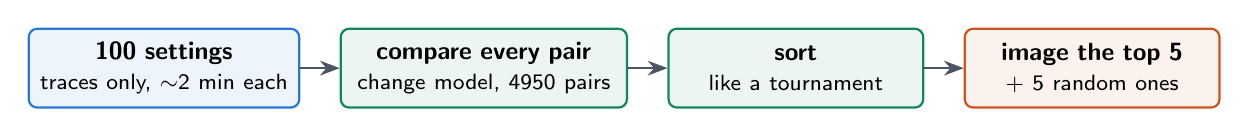
\begin{tikzpicture}[node distance=0.5cm]
\node[box=trace,text width=3.2cm] (a) {\textbf{100 settings}\\\footnotesize traces only, $\sim$2 min each};
\node[box=model,right=of a,text width=3.4cm] (b) {\textbf{compare every pair}\\\footnotesize change model, 4950 pairs};
\node[box=model,right=of b,text width=3.0cm] (c) {\textbf{sort}\\\footnotesize like a tournament};
\node[box=image,right=of c,text width=3.0cm] (d) {\textbf{image the top 5}\\\footnotesize + 5 random ones};
\foreach \x/\y in {a/b,b/c,c/d} \draw[arr] (\x)--(\y);
\end{tikzpicture}}
\end{center}
Imaging 100 settings would take about 27 hours. Screening 100 with traces and imaging 10 takes about 7. Each
setting is screened with its own traces only, with no extra reference trace: we compare settings with each other,
not with nominal. This first round ranks by $\lambda$ only. A predicted $\sigma_e$ is attached to each pick afterwards
as a sanity check. The 5 random settings that are also imaged are the control: if the model's picks are not clearly
better than random picks, the funnel does not work.

\subsection{A worked example: sorting six settings}
\figw[0.75]{e_sort6}
\readit{Six first-night settings, A--F (L1\_10, L1\_13, L1\_17, L1\_21, L1\_18, L1\_29), on an amplifier the model never
saw. Each cell is the model's probability that the \emph{row} setting has lower $\lambda$ than the \emph{column}
setting. Blue = ``the row wins'', red = ``the row loses''. ``Wins'' adds up each row (5 = beats everyone). The last
column is the truth.}
\shows{B wins almost every comparison (4.5 of 5), and B is truly the best ($-34$\,\%). A loses almost every
comparison, and A is truly bad ($+27$\,\%). C, D and F tie in the middle, and truly they are within 10\,\% of each
other, so this is about right. The miss is E. Its true $\lambda$ is $+138$\,\%, but E is L1\_18, the packet that waited
38 minutes without a clear. Its bad $\lambda$ came from that wait, not from its setting, and the traces taken before
the wait could not know.}

\textbf{From wins to an order.} Counting wins already gives a good order. We use a refinement called
\textbf{Bradley--Terry} (the idea behind chess ratings): each setting gets a strength $p$, chosen so that
``A beats B'' happens with probability $p_A/(p_A+p_B)$ across all comparisons. Beating a strong setting then counts
more than beating a weak one, and one wrong comparison is outvoted by the many others. On the first night it gave
almost the same order as counting wins (rank correlation 0.85 vs 0.84). We also tried ranking by the average predicted
size of the changes. It was less robust (one large wrong prediction moves a setting far) and was dropped.

\subsection{The funnel replayed on the first night}
\figw[0.95]{e_replay_bars}
\readit{All 35 non-nominal first-night settings, placed left to right in the order the model put them (left = predicted
lowest $\lambda$). The bar height is each setting's TRUE change of $\lambda$ from nominal. If the model were perfect,
the bars would rise steadily from left to right. Blue: the 5 the model would image.}
\shows{The overall order is good: the low bars are on the left and the high ones on the right (rank correlation 0.85).
3 of the 5 picks are among the truly best 5 (all about 16\,\% below nominal). The single best setting ($-34$\,\%)
came 7th, just outside the shortlist. The tall bar at position 21 is again L1\_18, the packet that waited.}

\subsection{How many images do we need?}
\figw[0.7]{e_regret}
\readit{If we image the first $k$ settings in the model's order (blue), or $k$ random settings (grey, averaged over
many draws), how far is the best one we find from the truly best setting?}
\shows{Following the model is better than random at almost every $k$. With 5 images it is 18\,\% from the best (random:
21\,\%). With 7 it finds the best (random: still 18\,\% away). On this night 5 picks were slightly too few, so 7--10
would be safer. But this is one night with 35 settings, essentially \emph{one} trial. Session F in v2 is the real test.}

\subsection{The noise number attached to each pick}
\figw[0.5]{e_noise}
\readit{$\sigma_e$ predicted from a single trace (plus which amplifier) against the image's $\sigma_e$, for every
first-night row. Grey band: the typical error.}
\shows{The prediction is good to about 10\,\%. That is enough to warn that a pick would have bad noise (0.15 vs 0.20),
but not enough to rank settings whose noise differs by 3\,\%. So it is attached to the picks, not used to make them.}

\subsection{Later rounds: trading noise against dark charge}
Some knobs lower $\sigma_e$ but raise $\lambda$. Later rounds rank by a weighted mix,
\[J=w\cdot(\text{change of }\log\sigma_e)+(1-w)\cdot(\text{change of }\log\lambda),\]
where $w=0$ is ``dark charge only'' (the first round), $w=1$ is ``noise only'', and $w=0.5$ counts a given percentage
change of either the same. The same change model serves every $w$. After a round, the next one searches a smaller range
of settings around the best picks. That is level 2 (a person runs the rounds); level 3 is the same loop running by
itself.

% =====================================================================================================
\section{v2: what the next data taking is for}

\subsection{Level-1 strips: measure each amplifier's level in every packet}
A \textbf{strip} is a tiny image, 2 rows $\times$ 1000 pixels, read exactly like the real image (same prescan, same
clear, 500 skips), but at ``level 1'': every skip of every pixel is kept, not only the average.

\begin{center}\small
\begin{tabular}{lp{3.2cm}p{3.2cm}p{3.2cm}}\toprule
 & trace & \textbf{strip (new)} & image\\\midrule
pixels & 10 & 2000 & 32\,000\\
time & seconds & about 1/16 of an image & $\sim$10 min\\
sees electrons (gain) & \xmark & \cmark & \cmark\\
same readout path as the image & \xmark & \cmark & \cmark\\
every skip kept & \cmark & \cmark & \xmark\\\bottomrule
\end{tabular}
\end{center}

\textbf{Why it should fix the amplifier problem.} Section 4 showed the trace cannot give an amplifier's level,
because noise and gain cannot be separated without whole electrons. One measurement per amplifier fixed the level on
board 102. A strip \emph{is} that measurement, taken in every packet, at every setting: it resolves electrons, so it
measures this amplifier's gain, $\sigma_e$ and part of $\lambda$ directly. The model then only has to learn the small
difference between strip and image, which is about the readout, not about which amplifier it is. It also closes the
timing gap of section 3, because the strip goes through the same prescan and clear as the image.

\begin{caveat}
Limit: strip rows hardly wait, so a strip sees the charge added during readout but little of the dark current that
builds up while rows wait. That part of $\lambda$ still needs the image (32 rows in v2 instead of 16).
\end{caveat}

\subsection{Varying all knobs together}
\figw[0.7]{e_design}
\readit{Two of the twelve knobs, delayInt and VR1. Orange squares: first-night settings. Blue dots: v2 settings.}
\shows{The first night mostly changed one knob at a time: the points lie on the horizontal and vertical lines through
nominal (star). v2 spreads the settings over the whole space, with all twelve knobs moved together. This fixes three
problems at once. Testing becomes interpolation (section 3). Every knob takes 40--50 different values, so the models
can learn its effect. And pairs that differ in two kinds of knob, the weak spot of section 5, become common.}

\subsection{Every v2 change answers a first-night lesson}
\begin{center}\small
\begin{tabular}{p{7.2cm}p{8cm}}\toprule
first-night lesson & v2 change\\\midrule
one-knob packets made the training check misleading & all 12 knobs move together (a ``Sobol'' design)\\
the trace cannot measure an amplifier's level or gain & a reference strip and a new strip in every packet\\
$\lambda$ drifts and depends on history & clear right before every image; nominal every 7 packets\\
nominal reference $\Rightarrow$ 96\,\% ``worse'' & 21 packets compare with the previous packet's setting\\
label noise known only at nominal & 3 settings repeated later in the night\\
3 test packets lost all traces & traces checked on the spot, damaged ones retaken\\
the learning curve was still improving & 61 training packets instead of 32, plus 15 held out\\
the funnel needs a real test & session F: 100 screens, 5 picks, 5 random controls\\\bottomrule
\end{tabular}
\end{center}

\subsection{The plan}
\begin{center}
\resizebox{\linewidth}{!}{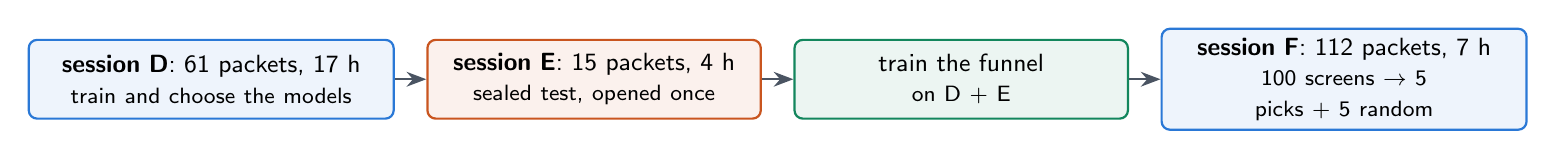
\begin{tikzpicture}[node distance=0.4cm]
\node[box=trace,text width=4.4cm] (d) {\textbf{session D}: 61 packets, 17 h\\\footnotesize train and choose the models};
\node[box=image,right=of d,text width=4.0cm] (e) {\textbf{session E}: 15 packets, 4 h\\\footnotesize sealed test, opened once};
\node[box=model,right=of e,text width=4.0cm] (m) {train the funnel\\\footnotesize on D + E};
\node[box=trace,right=of m,text width=4.4cm] (f) {\textbf{session F}: 112 packets, 7 h\\\footnotesize 100 screens $\to$ 5 picks + 5 random};
\foreach \x/\y in {d/e,e/m,m/f} \draw[arr] (\x)--(\y);
\end{tikzpicture}}
\end{center}

\subsection{What v2 should tell us, and what we do with each answer}
\begin{center}\small
\begin{tabular}{p{7.4cm}p{7.8cm}}\toprule
question & what we do with the answer\\\midrule
which predicts the image best: traces, strips, or both? & use the cheapest input that is good enough for each number\\
is the change between two traces predicted in size, or only in direction? & size: tune with a regression model; direction only: tune by ranking, as in the funnel\\
does it carry over to a new amplifier, and to another CCD? & yes: one model for all; no: a short calibration session per CCD\\
are the session-F picks clearly better than the random ones? & yes: screen with traces, image only the shortlist; no: keep imaging every candidate\\
is more data still helping? & yes: plan a third night\\\bottomrule
\end{tabular}
\end{center}

\subsection{What more data will and will not fix}
\textbf{Will help:} the errors were still falling with more packets ($\sigma_e$ 9.7 $\to$ 5.9\,\%, $\lambda$ 19 $\to$
10\,\% from 8 to 32 training packets). The comparison results were not yet statistically firm (50--120 clear changes),
and v2 gives thousands of pairs. The funnel replay was one trial, and session F is a second, independent one. Knobs
that barely moved anything on the first night (clock rails, VSUB) are now moved together with the rest.

\textbf{Will not help:} the trace's blindness to an amplifier's level (a physical limit, fixed by the strips), the
history dependence of $\lambda$ (fixed by the clearing routine, not by more packets), and whether the models carry
over to another CCD (only data from a second CCD can say).

% =====================================================================================================
\section{Conclusions}
\begin{enumerate}[leftmargin=1.4em]
\item A trace predicts the image's $\lambda$ (5\,\% vs 23\,\% without it) and $\sigma_e$ (7 vs 10\,\%) on amplifiers
  the model knows. The best model is the one built on the physics of the readout.
\item Much of that for $\lambda$ and gain is recognising the amplifier. A trace cannot give an amplifier's level,
  because noise and gain look the same in it.
\item Comparing two traces of the same amplifier removes the level. The direction of a change is right 75--90\,\% of
  the time on amplifiers never seen.
\item Sorting 35 settings by pairwise comparisons from traces alone gives a good order (0.85). The best setting was 7th
  of 35, so a shortlist of 7--10 would be safer than 5.
\item The realistic product of level 1 is a \textbf{comparator}: ``is setting B better than A for this amplifier?'' from
  two short traces, plus one measured level per amplifier from a strip. v2 is designed to test exactly that, and session
  F tests the funnel built on it.
\end{enumerate}

\appendix
\section{Every model tried, in one table}
\small
\begin{tabular}{p{3.4cm}p{6.8cm}p{4.8cm}}\toprule
model & what it does & verdict\\\midrule
\multicolumn{3}{l}{\textit{No trace (baselines)}}\\
mean, amplifier mean & guess the average (of that amplifier) & reference\\
settings GP / trees & predict from the settings only & reference\\
settings + amplifier & settings and which amplifier; the fair baseline & beaten for $\lambda$\\[2pt]
\multicolumn{3}{l}{\textit{Built on the physics of the readout}}\\
physics\_white & $\sigma_e$ = measured white noise $/\sqrt{500}/$gain + small learned correction & \textbf{best on the sealed test}\\
physics (Allan) & the same with a slow-noise floor that jumps between packets & failed for $\sigma_e$ (30\,\%)\\
physics\_joint, \_hier, sets, physics\_cnn & variants (joint targets, per-amplifier levels, CNN inputs) & no better\\[2pt]
\multicolumn{3}{l}{\textit{Flexible machine learning on the 141 features}}\\
boosted trees & sums of many small decision trees & good on known amplifiers\\
gp, gp\_dim, gp\_saas & Gaussian processes (smooth interpolation) & gp\_dim best in training, worst on the test\\
nn & neural network on the features & good on known amplifiers\\
ridge & linear & unstable\\[2pt]
\multicolumn{3}{l}{\textit{Networks on the 16 curves}}\\
cnn, pretrained cnn, deep kernel & learn their own features from the curves & mixed; best $\lambda$ on a new amplifier (cnn)\\[2pt]
\multicolumn{3}{l}{\textit{Change models (two traces)}}\\
trees on B $-$ A & feature differences & good\\
trees on [A, B, B $-$ A] & both traces and their difference & \textbf{best}\\
hand-picked bands + GP & selected parts of the difference curves & adds nothing\\
shared-encoder network & the same network applied to A and B & overfits\\
direction classifier & ``is B worse?'' with noise-sized changes down-weighted & \textbf{used for ranking}\\\bottomrule
\end{tabular}
\normalsize

\vspace{1em}
{\sloppy\textit{Sources: the first-data report (docs/overleaf\_first\_data\_2026-11-03), the level-1 summary
(docs/overleaf\_overview\_2026-11-04), the scorecard and ranking reports (docs/scorecard\_2026-11-04), the funnel replay
(lvl1/funnel\_replay.py), the v2 plan (docs/overleaf\_v2\_training\_plan\_2026-11-04). Figures:
docs/slides/make\_explained\_2026\_11\_05.py.}\par}

\end{document}
